\documentclass[fr]{../../../../../eplexam}

\usepackage{../../math-exam}
\usepackage{../../../../../eplunits}

\newcommand{\X}[1]{\ifthenelse{\equal{#1}{true}}{X}{}}

\newcommand{\vraioufaux}[1]{
  \begin{center}
    \begin{tabular}{p{0.7\textwidth}|c|c|}
      $+1$ point si bonne réponse, $-0.5$ point si mauvaise réponse,
      0 point si abstention & Vrai & Faux\\
      \hline
      (a) L'EDP a un caractère convectif et diffusif:&\X{#1}&\\
      (b) Le problème de condition initiale, avec $u(s, 0) = f(s)$ donné,
      est toujours bien posé:&\X{#1}&\\
      Supposons, pour la suite, le problème bien posé. Alors,&&\\
      (c) on ne peut trouver la solution que pour $t \geq 0$:&\X{#1}&\\
      (d) $I(t)=\int_{-\infty}^{\infty} u(x,t)\dif x$ est
      conservée au cours du temps:&\X{#1}&\\
    \end{tabular}
  \end{center}
}

\hypertitle{Math\'ematique}{3}{FSAB}{1103}{2013}{Janvier}
{Legat Beno\^it}
{Jean-François Remacle et Grégoire Winckelmans}

\section*{Question 1}
Considérons l'EDP suivante pour $u(x,t)$:
\[ \fpart{u}{t} + \fpart{(cu)}{x} =
\fpart{}{x}\left(\alpha\fpart{u}{x}\right) \]
avec $\alpha = \alpha(x) > 0$ et avec $c = c(x)$.\\
On considère d'abord un \textbf{problème en milieu infini}
($-\infty < x < \infty$) et avec $u\to 0$ à l'infini.\\
Répondre directement dans le tableau avec des ``X'':

\vraioufaux{false}

On considère ensuite un \textbf{problème en milieu semi-infini}
($0 \leq x < \infty$) et pour l'EDP avec $\alpha = 0$.
On a $c(x) = c_0\exp\left(-\frac{x}{L}\right)$,
avec $c_0$ et $L$ constants.
La condition limite est $u(0,t) = 0$.
La condition initiale pour $s \geq 0$ est
$u(s,0) = u_0\frac{s}{B}\left(1-\frac{s}{B}\right)$,
avec $u_0$ et $B$ constants.
\begin{enumerate}
  \item Prouvez que $I(t)=\int_0^\infty u(x, t) \dif x$
    est ici conservée au cours du temps.
  \item Obtenez le réseau des caractéristiques:
    équation et esquisse (propre, et avec axes chiffrés!)
    dans la partie supérieure droite du plan.
    Déterminez graphiquement la région où $u(x,t)$ est nulle.
  \item Obtenez l'expression de la solution dans la région où
    $u(x,t)$ n'est pas nulle.
\end{enumerate}

\solution{

  \vraioufaux{true}

  \begin{enumerate}[a)]
    \item C'est une équation de transport conservative.
    \item \label{en:pos}
      C'est vrai pour les temps $> 0$,
      en temps $< 0$ ca ne fonctionne plus puisqu'on
      a une déformation de l'onde.
    \item Ça découle de la \ref{en:pos}).
    \item C'est expliqué dans le syllabus.
  \end{enumerate}

  L'EDP devient
  \begin{align*}
    \fpart{u}{t} + \fpart{(cu)}{x} & = 0\\
    \fpart{u}{t} + c\fpart{u}{x} & = -u\fpart{c}{x}\\
    \fpart{u}{t} + c\fpart{u}{x} & = u\frac{c_0}{L}e^{-\frac{x}{L}}
  \end{align*}
  \begin{enumerate}
    \item On a
      \begin{align*}
        \fpart{}{t}\int_0^\infty u \dif x
        & = \int_0^\infty \fpart{u}{t} \dif x\\
        & = \int_0^\infty -\fpart{(cu)}{x} \dif x\\
        & = [-cu]_0^\infty.
      \end{align*}
      Seulement, par l'énoncé, on a $u(0, t) = 0$ et
      $\lim_{x\to\infty} cu = 0$ donc $u$ est bien
      indépendant de $t$.
    \item On a
      \[ \dif x = c(x) \dif t \]
      ou encore
      \[ \frac{e^{\frac{x}{L}}}{c_0}\dif x = \dif t \]
      d'où
      \begin{align}
        \nonumber
        \int_s^x \frac{e^{\frac{x'}{L}}}{c_0}\dif x' = \int_0^t \dif t'\\
        \label{eq:cara}
        \frac{L}{c_0}\left(e^{\frac{x}{L}}-e^{\frac{s}{L}}\right) = t
      \end{align}
      Le long de ces caractéristique, on a
      \[ \fdif{u}{t} = u\frac{c_0}{L}e^{\frac{-x}{L}} \]
      quand $u$ vaut 0 au début de la caractéristique,
      $\fdif{u}{t}$ vaudra 0 au début aussi et $u$ n'augmentera alors pas,
      il restera donc 0, $\fdif{u}{t}$ restera donc aussi 0 et de proche
      en proche, on aura $u = 0$ tout le long de cette caractéristique.
      Comme $u(0, t) = 0$, toute la partie en rouge
      sur la figure~\ref{fig:cara} a $u = 0$.
      $u$ vaut aussi 0 le long de la caractéristique passant par $s = B$
      car $u(B, 0) = u_0\frac{B}{B}\left(1-\frac{B}{B}\right) = 0$.
      \begin{figure}
        \centering
        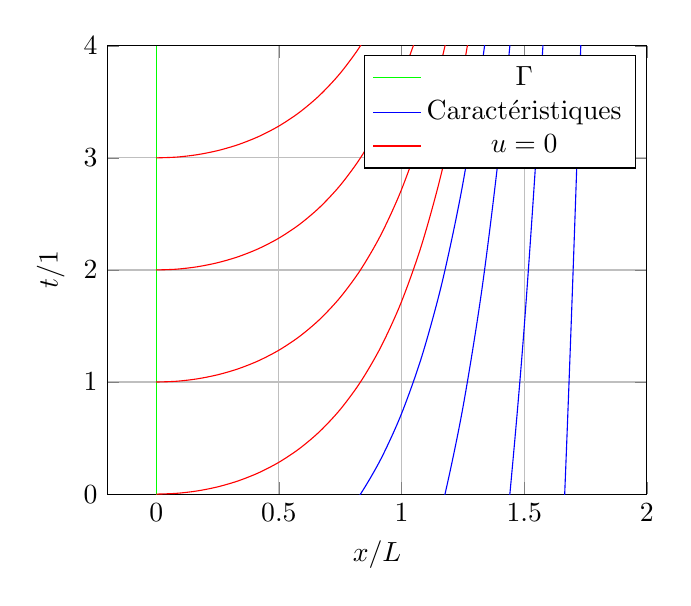
\begin{tikzpicture}
          \begin{axis}[xmax=2,ymin=0,ymax=4,
              xlabel = {$x/L$},
            ylabel = {$t/\si{1}{\second}$}, grid]
            \addplot[green,smooth] plot coordinates {(0,-4) (0,4)};
            \addlegendentry{$\Gamma$};
            \addplot[blue,smooth,domain=0:2]{exp(x^2)-2};
            \addlegendentry{Caractéristiques};
            \addplot[red,smooth,domain=0:2]{exp(x^2)-1};
            \addlegendentry{$u = 0$};
            \addplot[blue,smooth,domain=0:2]{exp(x^2)-4};
            \addplot[blue,smooth,domain=0:2]{exp(x^2)-8};
            \addplot[blue,smooth,domain=0:2]{exp(x^2)-16};
            \addplot[red,smooth,domain=0:2]{exp(x^2)};
            \addplot[red,smooth,domain=0:2]{exp(x^2)+1};
            \addplot[red,smooth,domain=0:2]{exp(x^2)+2};
          \end{axis}
        \end{tikzpicture}
        \caption{Caractéristiques et $\Gamma\equiv t = 0$.}
        \label{fig:cara}
      \end{figure}
    \item Sur les caractéristiques, en utilisant \eqref{eq:cara}, on a
    \begin{align*}
      u\frac{c_0}{L}e^{-\frac{x}{L}}\dif t & = \dif u\\
      \frac{\dif t}{t+\frac{L}{c_0}e^{\frac{s}{L}}} & = \frac{\dif u}{u}\\
      \int_0^t \frac{\dif t'}{t'+\frac{L}{c_0}e^{\frac{s}{L}}}
      & = \int_{u(s,0)}^{u}\frac{\dif u'}{u'}\\
      \ln\left(
      \frac{t+\frac{L}{c_0}e^{\frac{s}{L}}}{\frac{L}{c_0}e^{\frac{s}{L}}}
      \right)
      & = \ln\left(\frac{u}{u(s,0)}\right)\\
      \frac{\frac{L}{c_0}e^{\frac{x}{L}}}{\frac{L}{c_0}e^{\frac{x}{L}}-t}
      & = \frac{u}{u(s,0)}\\
      \frac{u(s,0)}{1-t\frac{c_0}{L}e^{-\frac{x}{L}}}
      & = u.
    \end{align*}
    Seulement, on a, par \eqref{eq:cara}
    \[ s = L\ln\left(e^{\frac{x}{L}}-\frac{c_0}{L}t\right) \]
    donc
    \[ u = u_0 \frac{L}{B}\ln\left(e^{\frac{x}{L}}-\frac{c_0}{L}t\right)
      \frac{1-\frac{L}{B}\ln\left(e^{\frac{x}{L}}-\frac{c_0}{L}t\right)}
    {1-t\frac{c_0}{L}e^{-\frac{x}{L}}}. \]
\end{enumerate}}

\section*{Question 2}
On considère l'EDP suivante pour $u(x,t)$:
\[ \fpart{u}{t} = \alpha\ffpart{u}{x} \]
avec $\alpha>0$. Le domaine est borné: $0\leq x \leq L$.
La condition initiale est
$u(x,0) = u_0\left(1 - \frac{x}{L}\right)$ avec $u_0$ constant.
Pour $t > 0$, on impose que $\fpart{u}{x}(0,t) = -\frac{u_0}{2L}$ et
que $u(L,t) = 0$.

La solution du problème est de la forme
$u(x, t) = R(x) + \Theta(x, t)$ avec $R$ la solution
de régime et $\Theta$ la solution transitoire.

\begin{enumerate}
  \item Obtenez d'abord $R$.
  \item Esquissez alors l'évolution ``attendue'' (pas de calcul,
    esquisse propre!) de la solution:
    graphe de $\frac{u}{u_0}$ en fonction de $\frac{x}{L}$ pour
    un ``temps court'', et aussi pour un ``temps moyen''.\\
    Mathématiquement, qu'est-ce qu'un ``temps court''
    pour cette EDP?
  \item Obtenez finalement $\Theta$, par séparatio des variables
    (écrivez clairement les intégrales à effectuer pour obtenir
    les coefficients du développement en série,
    mais ne les effectuez pas).
\end{enumerate}
\solution{
  \begin{enumerate}
    \item
      En $t \to \infty$, on a $\Theta \to 0$.
      Comme $R$ est indépendant du temps, il doit respecter les conditions
      aux limites tout seul. Il doit aussi respecter l'EDP donc
      \[ \alpha\ffpart{R}{x} = \fpart{R}{t} = 0 \]
      d'où on trouve que $\exists A, B \in \mathbb{R}$.
      \[ R(x) = Ax + B. \]
      Comme $R'(0) = -\frac{u_0}{2L}$ et $R(L) = 0$, on a
      \[ R(x) = \frac{u_0}{2}\left(1-\frac{x}{L}\right). \]
    \item
      \begin{figure}
        \centering
        %\begin{subfigure}[b]{0.4\textwidth}
          %\centering
        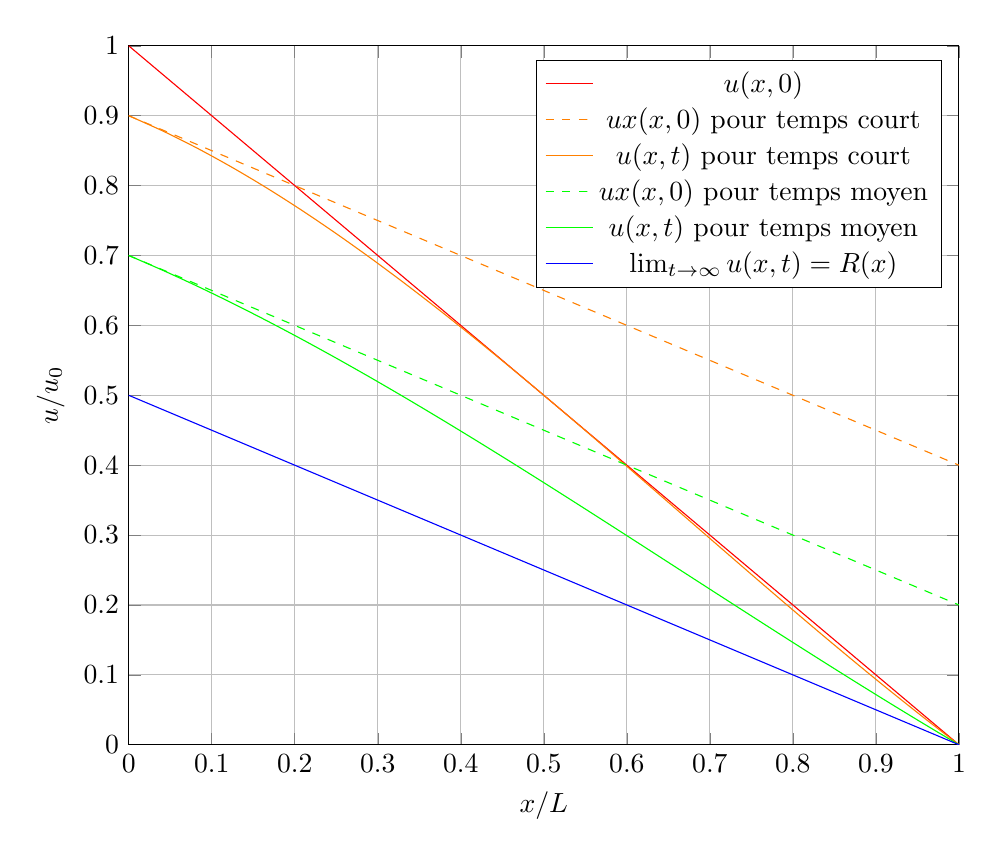
\begin{tikzpicture}
          \begin{axis}[ymin=0,xmin=0,xmax=1,ymax=1,
              xlabel = {$x/L$},width={\textwidth},
            ylabel = {$u/u_0$}, grid]
              %\addplot[green,smooth] plot coordinates {(0,-4) (0,4)};
              %\addlegendentry{$\Gamma$};
            \addplot[red,smooth,domain=0:1]{1-x};
            \addlegendentry{$u(x,0)$};
            \addplot[orange,smooth,dashed,domain=0:1]{0.5*(1.8-x)};
            \addlegendentry
            {$\fpart{u}{x}(x,0)$ pour temps court};
            \addplot[orange,smooth,domain=0:1] % aah spline cubiques :)
            {0.4*x^3 -0.8*x^2 -0.5*x  +0.9};%f'(1)=-0.9
              %{0.425*x^3  -0.825*x^2 -0.5*x  +0.9};%f''(1) = 0.9
              %{0.45*x^3  -0.85*x^2 -0.5*x  +0.9};
              %{0.5*x^3  -0.9*x^2 -0.5*x  +0.9};
              %{-0.4*x^2-0.5*x+0.9};
            \addlegendentry{$u(x,t)$ pour temps court};
            \addplot[green,smooth,dashed,domain=0:1]{0.5*(1.4-x)};
            \addlegendentry
            {$\fpart{u}{x}(x,0)$ pour temps moyen};
            \addplot[green,smooth,domain=0:1] % aah spline cubiques :)
            {0.2*x^3 -0.4*x^2 -0.5*x  +0.7};%f'(1)=-0.7
              %{0.275*x^3  -0.475*x^2 -0.5*x  +0.7};%f''(1) = 0.7
            \addlegendentry{$u(x,t)$ pour temps moyen};
            \addplot[blue,smooth,domain=0:1]{0.5*(1-x)};
            \addlegendentry{$\lim_{t\to\infty}u(x,t) = R(x)$};
          \end{axis}
        \end{tikzpicture}
        \caption{Solution pour temps court et long.}
        \label{fig:time}
      \end{figure}
      Les dessins sont représentés sur la figure~\ref{fig:time}.
      Un temps court est un temps pour lequel,
      la solution transitoire $\Theta$
      est encore loin d'être négligeable, c'est à dire que
      $t < \frac{\alpha}{L^2}$.
    \item Soit $\Theta = X(x) T(t)$, on a
      \[ \alpha \frac{X''}{X} = \frac{T'}{T} = 0. \]
      Aux limites, on a $\fpart{\Theta}{x}(0,t) = \fpart{u}{x}(0,t) -
      R'(0) = 0$ et $\Theta(L,t) = u(L,t) - R(L) = 0$.
      Comme les conditions aux limites en $x$ sont homogènes,
      $k^2$ nous donnera la solution trivial. $k = 0$ nous redonne $R$.
      Il faut donc considérer uniquement $\frac{X''}{X} = -k^2$.
      Ce qui donne $\exists C, D \in \mathbb{R}$ tels que
      \[ X(x) = C\cos(kx) + D\sin(kx). \]
      Avec $\fpart{\Theta}{x}(0,t) = 0$, on a
      \[ 0 = T(t)(-C\sin(0) + D\cos(0)) = T(t)D. \]
      Comme on ne veut pas la solution triviale, $\exists t$ tel que
      $T(t) \neq 0$ donc $D = 0$.
      $\Theta(L,t) = 0$ nous donne
      \[ T(t)C\cos(kL) = 0. \]
      Comme on ne veut pas la solution triviale, $C \neq 0$ et
      $\exists t$ tel que $T(t) \neq 0$ donc $\cos(kL) = 0$ d'où
      $\exists n \in \mathbb{Z}_{>0}$ tel que
      \[ k_n = \left(n-\frac{1}{2}\right)\frac{\pi}{L}. \]
      On a alors pour $T$
      \[ T' = -\alpha k_n^2 T \]
      d'où $T(t) = E_ne^{-\alpha k_n^2 t}$ donc, avec $F_n = E_nC_n$,
      \[ \Theta(x,t) = \sum_{n=1}^\infty F_ne^{-\alpha k_n^2 t}
      \cos(k_nx) \]
      La condition sur $u(x,0)$ nous donne
      \begin{align*}
        \Theta(x,0) & = u(x,0) - R(x)\\
        \sum_{n=1}^\infty F_ne^{-\alpha k_n^2 0} \cos(k_nx)
        & = u_0\left(1-\frac{x}{L}\right) -
        \frac{u_0}{2}\left(1-\frac{x}{L}\right)\\
        \sum_{n=1}^\infty F_n \cos(k_nx)
        & = \frac{u_0}{2}\left(1-\frac{x}{L}\right).
      \end{align*}
      Par l'orthogonalité des cosinus, on a
      \[ F_m
        = \frac{u_0}{L}\int_0^L \left(1-\frac{x}{L}\right) \cos(k_m x)
      \dif x. \]
  \end{enumerate}
}

\section*{Question 3}
On définit la fonction:
\begin{align*}
  w & = \arctan(z) = \int_0^z \frac{\dif\tilde{z}}{1+\tilde{z}}
  = \frac{i}{2}\log\left(\frac{i+z}{i-z}\right) & z \neq \pm i.
\end{align*}
\begin{enumerate}
  \item Obtenez les points de branchement de $w$.
    Proposez un choix de coupures
    (pour la suite, on utilisera la branche principale).
  \item Vérifiez que la définition de $w$ est bien telle que $\tan w = z$.
  \item Obtenez l'expression de $w$ pour $z = iy$
    avec $-1 < y < 1$.
    À partir de ce résultat,
    obtenez aussi l'expression de $\arctanh y$.
  \item Obtenez le développement en série de $w$ autour de $z_0=0$
    Quel est le rayon de convergence de cette série?
\end{enumerate}
\rappelscomplexes

\solution{
  \begin{enumerate}
    \item
      On remarque tout de suite qu'on annule le $\log$ en $z=-i$ mais c'est
      pas clair si $i$ est un point de branchement ou pas.
      Seulement, en développant
      \[ \arctan(z) = \frac{i}{2}(\log(i+z) - \log(i-z)), \]
      on voit que $i$ annule aussi un $\log$ et est donc aussi un point
      de branchement.
      Les deux seuls points de branchement sont donc $\pm i$.
      Une coupure possible est $-\frac{\pi}{2} \leq \theta_1 < 3\frac{\pi}{2}$
      et $\frac{\pi}{2} \leq \theta_2 < \frac{5\pi}{2}$ où
      $\theta_1$ est l'angle par rapport à $-i$ et $\theta_2$ l'angle
      par rapport à $+i$.
    \item On a successivement
      \begin{align*}
        \tan(w) & = \frac{\sin(w)}{\cos(w)}\\
        & = -i\frac{e^{iw}-e^{-iw}}{e^{iw}+e^{-iw}}\\
        & = i\frac{e^{-2iw}-1}{e^{-2iw}+1}\\
        & = i\frac{\frac{i+z}{i-z}-1}{\frac{i+z}{i-z}+1}\\
        & = i\frac{i+z-i+z}{i+z+i-z}\\
        & = i\frac{2z}{2i}\\
        & = z.
      \end{align*}
    \item On a successivement
      \begin{align*}
        \arctan(iy) & = \frac{i}{2}\log\left(\frac{i+z}{i-z}\right)\\
        & = \frac{i}{2}\log\left(\frac{i+iy}{i-iy}\right)\\
        & = \frac{i}{2}\log\left(\frac{1+y}{1-y}\right).
      \end{align*}
      De plus, on a
      \[ \tan(z) = \frac{\sin(z)}{\cos(z)} = -i\frac{\sinh(iz)}{\cosh(iz)}
      = -i\tanh(iz). \]
      En posant $z = \arctan(-iy)$, on a
      \[ -iy = -i\tanh(iz) \]
      d'où
      \[ y = \tanh(iz) \]
      et donc
      \[ \arctanh(y) = iz = i\arctan(-iy) =
      -\frac{1}{2}\log\left(\frac{1-y}{1+y}\right) =
      \frac{1}{2}\log\left(\frac{1+y}{1-y}\right). \]
  \end{enumerate}
}

\section*{Question 4}
Calculez l'intégrale suivante:
\[ I = \int_0^{2\pi}\frac{\cos(2\theta)}{5 - 4\cos(\theta)}\dif \theta. \]
en utilisant le théorème des résidus.

\solution{
  On a successivement, en définissant $C$ comme étant
  un cercle de rayon 1 et de centre 0 dans le plan complexe,
  \begin{align*}
  \int_0^{2\pi}\frac{\cos(2\theta)}{5 - 4\cos(\theta)}\dif \theta
  &= \oint_C \frac{\frac{z^2+z^{-2}}{2}}
  {5 - 4\frac{z+z^{-1}}{2}}\frac{\dif z}{iz}\\
  &= -\frac{1}{2i}\oint_C \frac{z^4+1}
  {z^2(2z^2-5z+2)}\dif z\\
  &= -\frac{1}{2i}\oint_C \frac{z^4+1}
  {z^2(2z-1)(z-2)}\dif z\\
  \end{align*}
  Soit $f(z)$ l'intégrant de la dernière intégrale.
  On voit que $f$ a 3 pôles: 0 de degré 2, $\frac{1}{2}$ de degré 1
  et 2 de degré 1.
  On sait calculer
  \begin{align*}
    \res(f,0) & = \frac{1}{1!}\left.\fdif{z^2f}{z}\right|_{z = 0}\\
    & = \left.\frac{4z^3(2z-1)(z-2)-(z^4+1)(4z-5)}
    {(2z-1)^2(z-2)^2}\right|_{z = 0}\\
    & = \frac{5}{4}\\
    \res\left(f,\frac{1}{2}\right)
    & = \frac{1}{0!}\lim_{z\to\frac{1}{2}}\left(z-\frac{1}{2}\right)f\\
    & = \frac{\frac{1}{16} + 1}{2\frac{1}{4}\left(\frac{1}{2}-2\right)}\\
    & = -\frac{17}{12}
  \end{align*}
  \paragraph{Attention} C'est primordial de multiplier
  par $z-\frac{1}{2}$ et non par $2z-1$, beaucoup ont fait la faute et
  arrive à $\pi\frac{19}{12}$ à la place de $\frac{\pi}{6}$.

  Par le théorème des Résidus, comme 2 est en dehors de $C$,
  \begin{align*}
    I & = -\frac{1}{2i}\oint_C \frac{z^4+1}{z^2(2z-1)(z-2)}\dif z\\
    &= -\frac{1}{2i}2\pi i
    \left(\res(f,0)+\res\left(f,\frac{1}{2}\right)\right)\\
    &= -\pi\left(\frac{5}{4}-\frac{17}{12}\right)\\
    &= \frac{\pi}{6}.
  \end{align*}
}

\end{document}
